\documentclass[1p]{elsarticle_modified}
%\bibliographystyle{elsarticle-num}

%\usepackage[colorlinks]{hyperref}
%\usepackage{abbrmath_seonhwa} %\Abb, \Ascr, \Acal ,\Abf, \Afrak
\usepackage{amsfonts}
\usepackage{amssymb}
\usepackage{amsmath}
\usepackage{amsthm}
\usepackage{scalefnt}
\usepackage{amsbsy}
\usepackage{kotex}
\usepackage{caption}
\usepackage{subfig}
\usepackage{color}
\usepackage{graphicx}
\usepackage{xcolor} %% white, black, red, green, blue, cyan, magenta, yellow
\usepackage{float}
\usepackage{setspace}
\usepackage{hyperref}

\usepackage{tikz}
\usetikzlibrary{arrows}

\usepackage{multirow}
\usepackage{array} % fixed length table
\usepackage{hhline}

%%%%%%%%%%%%%%%%%%%%%
\makeatletter
\renewcommand*\env@matrix[1][\arraystretch]{%
	\edef\arraystretch{#1}%
	\hskip -\arraycolsep
	\let\@ifnextchar\new@ifnextchar
	\array{*\c@MaxMatrixCols c}}
\makeatother %https://tex.stackexchange.com/questions/14071/how-can-i-increase-the-line-spacing-in-a-matrix
%%%%%%%%%%%%%%%

\usepackage[normalem]{ulem}

\newcommand{\msout}[1]{\ifmmode\text{\sout{\ensuremath{#1}}}\else\sout{#1}\fi}
%SOURCE: \msout is \stkout macro in https://tex.stackexchange.com/questions/20609/strikeout-in-math-mode

\newcommand{\cancel}[1]{
	\ifmmode
	{\color{red}\msout{#1}}
	\else
	{\color{red}\sout{#1}}
	\fi
}

\newcommand{\add}[1]{
	{\color{blue}\uwave{#1}}
}

\newcommand{\replace}[2]{
	\ifmmode
	{\color{red}\msout{#1}}{\color{blue}\uwave{#2}}
	\else
	{\color{red}\sout{#1}}{\color{blue}\uwave{#2}}
	\fi
}

\newcommand{\Sol}{\mathcal{S}} %segment
\newcommand{\D}{D} %diagram
\newcommand{\A}{\mathcal{A}} %arc


%%%%%%%%%%%%%%%%%%%%%%%%%%%%%5 test

\def\sl{\operatorname{\textup{SL}}(2,\Cbb)}
\def\psl{\operatorname{\textup{PSL}}(2,\Cbb)}
\def\quan{\mkern 1mu \triangleright \mkern 1mu}

\theoremstyle{definition}
\newtheorem{thm}{Theorem}[section]
\newtheorem{prop}[thm]{Proposition}
\newtheorem{lem}[thm]{Lemma}
\newtheorem{ques}[thm]{Question}
\newtheorem{cor}[thm]{Corollary}
\newtheorem{defn}[thm]{Definition}
\newtheorem{exam}[thm]{Example}
\newtheorem{rmk}[thm]{Remark}
\newtheorem{alg}[thm]{Algorithm}

\newcommand{\I}{\sqrt{-1}}
\begin{document}

%\begin{frontmatter}
%
%\title{Boundary parabolic representations of knots up to 8 crossings}
%
%%% Group authors per affiliation:
%\author{Yunhi Cho} 
%\address{Department of Mathematics, University of Seoul, Seoul, Korea}
%\ead{yhcho@uos.ac.kr}
%
%
%\author{Seonhwa Kim} %\fnref{s_kim}}
%\address{Center for Geometry and Physics, Institute for Basic Science, Pohang, 37673, Korea}
%\ead{ryeona17@ibs.re.kr}
%
%\author{Hyuk Kim}
%\address{Department of Mathematical Sciences, Seoul National University, Seoul 08826, Korea}
%\ead{hyukkim@snu.ac.kr}
%
%\author{Seokbeom Yoon}
%\address{Department of Mathematical Sciences, Seoul National University, Seoul, 08826,  Korea}
%\ead{sbyoon15@snu.ac.kr}
%
%\begin{abstract}
%We find all boundary parabolic representation of knots up to 8 crossings.
%
%\end{abstract}
%\begin{keyword}
%    \MSC[2010] 57M25 
%\end{keyword}
%
%\end{frontmatter}

%\linenumbers
%\tableofcontents
%
\newcommand\colored[1]{\textcolor{white}{\rule[-0.35ex]{0.8em}{1.4ex}}\kern-0.8em\color{red} #1}%
%\newcommand\colored[1]{\textcolor{white}{ #1}\kern-2.17ex	\textcolor{white}{ #1}\kern-1.81ex	\textcolor{white}{ #1}\kern-2.15ex\color{red}#1	}

{\Large $\underline{12a_{0464}~(K12a_{0464})}$}

\setlength{\tabcolsep}{10pt}
\renewcommand{\arraystretch}{1.6}
\vspace{1cm}\begin{tabular}{m{100pt}>{\centering\arraybackslash}m{274pt}}
\multirow{5}{120pt}{
	\centering
	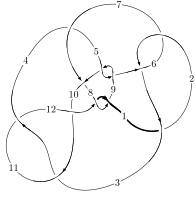
\includegraphics[width=112pt]{../../../GIT/diagram.site/Diagrams/png/1265_12a_0464.png}\\
\ \ \ A knot diagram\footnotemark}&
\allowdisplaybreaks
\textbf{Linearized knot diagam} \\
\cline{2-2}
 &
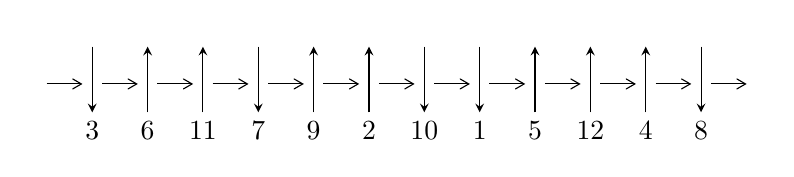
\begin{tikzpicture}[x=20pt, y=17pt]
	% nodes
	\node (C0) at (0, 0) {};
	\node (C1) at (1, 0) {};
	\node (C1U) at (1, +1) {};
	\node (C1D) at (1, -1) {3};

	\node (C2) at (2, 0) {};
	\node (C2U) at (2, +1) {};
	\node (C2D) at (2, -1) {6};

	\node (C3) at (3, 0) {};
	\node (C3U) at (3, +1) {};
	\node (C3D) at (3, -1) {11};

	\node (C4) at (4, 0) {};
	\node (C4U) at (4, +1) {};
	\node (C4D) at (4, -1) {7};

	\node (C5) at (5, 0) {};
	\node (C5U) at (5, +1) {};
	\node (C5D) at (5, -1) {9};

	\node (C6) at (6, 0) {};
	\node (C6U) at (6, +1) {};
	\node (C6D) at (6, -1) {2};

	\node (C7) at (7, 0) {};
	\node (C7U) at (7, +1) {};
	\node (C7D) at (7, -1) {10};

	\node (C8) at (8, 0) {};
	\node (C8U) at (8, +1) {};
	\node (C8D) at (8, -1) {1};

	\node (C9) at (9, 0) {};
	\node (C9U) at (9, +1) {};
	\node (C9D) at (9, -1) {5};

	\node (C10) at (10, 0) {};
	\node (C10U) at (10, +1) {};
	\node (C10D) at (10, -1) {12};

	\node (C11) at (11, 0) {};
	\node (C11U) at (11, +1) {};
	\node (C11D) at (11, -1) {4};

	\node (C12) at (12, 0) {};
	\node (C12U) at (12, +1) {};
	\node (C12D) at (12, -1) {8};
	\node (C13) at (13, 0) {};

	% arrows
	\draw[->,>={angle 60}]
	(C0) edge (C1) (C1) edge (C2) (C2) edge (C3) (C3) edge (C4) (C4) edge (C5) (C5) edge (C6) (C6) edge (C7) (C7) edge (C8) (C8) edge (C9) (C9) edge (C10) (C10) edge (C11) (C11) edge (C12) (C12) edge (C13) ;	\draw[->,>=stealth]
	(C1U) edge (C1D) (C2D) edge (C2U) (C3D) edge (C3U) (C4U) edge (C4D) (C5D) edge (C5U) (C6D) edge (C6U) (C7U) edge (C7D) (C8U) edge (C8D) (C9D) edge (C9U) (C10D) edge (C10U) (C11D) edge (C11U) (C12U) edge (C12D) ;
	\end{tikzpicture} \\
\hhline{~~} \\& 
\textbf{Solving Sequence} \\ \cline{2-2} 
 &
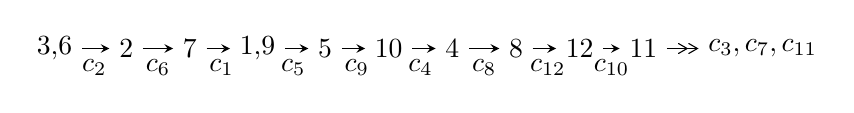
\begin{tikzpicture}[x=23pt, y=7pt]
	% node
	\node (A0) at (-1/8, 0) {3,6};
	\node (A1) at (1, 0) {2};
	\node (A2) at (2, 0) {7};
	\node (A3) at (49/16, 0) {1,9};
	\node (A4) at (33/8, 0) {5};
	\node (A5) at (41/8, 0) {10};
	\node (A6) at (49/8, 0) {4};
	\node (A7) at (57/8, 0) {8};
	\node (A8) at (65/8, 0) {12};
	\node (A9) at (73/8, 0) {11};
	\node (C1) at (1/2, -1) {$c_{2}$};
	\node (C2) at (3/2, -1) {$c_{6}$};
	\node (C3) at (5/2, -1) {$c_{1}$};
	\node (C4) at (29/8, -1) {$c_{5}$};
	\node (C5) at (37/8, -1) {$c_{9}$};
	\node (C6) at (45/8, -1) {$c_{4}$};
	\node (C7) at (53/8, -1) {$c_{8}$};
	\node (C8) at (61/8, -1) {$c_{12}$};
	\node (C9) at (69/8, -1) {$c_{10}$};
	\node (A10) at (11, 0) {$c_{3},c_{7},c_{11}$};

	% edge
	\draw[->,>=stealth]	
	(A0) edge (A1) (A1) edge (A2) (A2) edge (A3) (A3) edge (A4) (A4) edge (A5) (A5) edge (A6) (A6) edge (A7) (A7) edge (A8) (A8) edge (A9) ;
	\draw[->>,>={angle 60}]	
	(A9) edge (A10);
\end{tikzpicture} \\ 

\end{tabular} \\

\footnotetext{
The image of knot diagram is generated by the software ``\textbf{Draw programme}" developed by Andrew Bartholomew(\url{http://www.layer8.co.uk/maths/draw/index.htm\#Running-draw}), where we modified some parts for our purpose(\url{https://github.com/CATsTAILs/LinksPainter}).
}\phantom \\ \newline 
\centering \textbf{Ideals for irreducible components\footnotemark of $X_{\text{par}}$} 
 
\begin{align*}
I^u_{1}&=\langle 
-9.04807\times10^{406} u^{147}-2.76096\times10^{407} u^{146}+\cdots+1.92577\times10^{408} b-2.23875\times10^{410},\\
\phantom{I^u_{1}}&\phantom{= \langle  }2.14793\times10^{409} u^{147}-3.51499\times10^{409} u^{146}+\cdots+1.34996\times10^{411} a-6.24570\times10^{412},\\
\phantom{I^u_{1}}&\phantom{= \langle  }u^{148}+2 u^{147}+\cdots+2531 u+701\rangle \\
I^u_{2}&=\langle 
-3146106 u^{35}+3876595 u^{34}+\cdots+1724315 b+7517731,\\
\phantom{I^u_{2}}&\phantom{= \langle  }10268268 u^{35}-15331195 u^{34}+\cdots+1724315 a-6015468,\;u^{36}- u^{35}+\cdots+u+1\rangle \\
\\
\end{align*}
\raggedright * 2 irreducible components of $\dim_{\mathbb{C}}=0$, with total 184 representations.\\
\footnotetext{All coefficients of polynomials are rational numbers. But the coefficients are sometimes approximated in decimal forms when there is not enough margin.}
\newpage
\renewcommand{\arraystretch}{1}
\centering \section*{I. $I^u_{1}= \langle -9.05\times10^{406} u^{147}-2.76\times10^{407} u^{146}+\cdots+1.93\times10^{408} b-2.24\times10^{410},\;2.15\times10^{409} u^{147}-3.51\times10^{409} u^{146}+\cdots+1.35\times10^{411} a-6.25\times10^{412},\;u^{148}+2 u^{147}+\cdots+2531 u+701 \rangle$}
\flushleft \textbf{(i) Arc colorings}\\
\begin{tabular}{m{7pt} m{180pt} m{7pt} m{180pt} }
\flushright $a_{3}=$&$\begin{pmatrix}1\\0\end{pmatrix}$ \\
\flushright $a_{6}=$&$\begin{pmatrix}0\\u\end{pmatrix}$ \\
\flushright $a_{2}=$&$\begin{pmatrix}1\\u^2\end{pmatrix}$ \\
\flushright $a_{7}=$&$\begin{pmatrix}u\\u^3+u\end{pmatrix}$ \\
\flushright $a_{1}=$&$\begin{pmatrix}u^2+1\\u^2\end{pmatrix}$ \\
\flushright $a_{9}=$&$\begin{pmatrix}-0.0159110 u^{147}+0.0260377 u^{146}+\cdots+169.631 u+46.2657\\0.0469842 u^{147}+0.143369 u^{146}+\cdots+405.801 u+116.252\end{pmatrix}$ \\
\flushright $a_{5}=$&$\begin{pmatrix}-0.0465841 u^{147}+0.0201408 u^{146}+\cdots+402.993 u+158.980\\0.0358114 u^{147}-0.0197006 u^{146}+\cdots-137.396 u-63.0475\end{pmatrix}$ \\
\flushright $a_{10}=$&$\begin{pmatrix}0.0771767 u^{147}+0.00610062 u^{146}+\cdots-296.017 u-141.082\\-0.0264258 u^{147}-0.144854 u^{146}+\cdots-324.224 u-93.6180\end{pmatrix}$ \\
\flushright $a_{4}=$&$\begin{pmatrix}-0.0342021 u^{147}+0.101606 u^{146}+\cdots+694.847 u+253.271\\0.0566151 u^{147}+0.0229606 u^{146}+\cdots+2.26931 u-8.50367\end{pmatrix}$ \\
\flushright $a_{8}=$&$\begin{pmatrix}-0.00994220 u^{147}+0.0634565 u^{146}+\cdots+316.174 u+101.369\\0.0609589 u^{147}+0.101110 u^{146}+\cdots+169.224 u+49.1741\end{pmatrix}$ \\
\flushright $a_{12}=$&$\begin{pmatrix}-0.0966279 u^{147}-0.101794 u^{146}+\cdots+97.6154 u+126.522\\0.166862 u^{147}+0.374460 u^{146}+\cdots+352.861 u+82.3272\end{pmatrix}$ \\
\flushright $a_{11}=$&$\begin{pmatrix}-0.271375 u^{147}-0.910200 u^{146}+\cdots-1670.53 u-564.206\\-0.0600355 u^{147}-0.137866 u^{146}+\cdots-183.561 u-47.5237\end{pmatrix}$\\&\end{tabular}
\flushleft \textbf{(ii) Obstruction class $= -1$}\\~\\
\flushleft \textbf{(iii) Cusp Shapes $= 0.537377 u^{147}+0.175293 u^{146}+\cdots+358.399 u-104.006$}\\~\\
\newpage\renewcommand{\arraystretch}{1}
\flushleft \textbf{(iv) u-Polynomials at the component}\newline \\
\begin{tabular}{m{50pt}|m{274pt}}
Crossings & \hspace{64pt}u-Polynomials at each crossing \\
\hline $$\begin{aligned}c_{1}\end{aligned}$$&$\begin{aligned}
&u^{148}+72 u^{147}+\cdots+11695261 u+491401
\end{aligned}$\\
\hline $$\begin{aligned}c_{2},c_{6}\end{aligned}$$&$\begin{aligned}
&u^{148}-2 u^{147}+\cdots-2531 u+701
\end{aligned}$\\
\hline $$\begin{aligned}c_{3},c_{11}\end{aligned}$$&$\begin{aligned}
&u^{148}-3 u^{147}+\cdots+448 u+79
\end{aligned}$\\
\hline $$\begin{aligned}c_{4}\end{aligned}$$&$\begin{aligned}
&u^{148}-11 u^{147}+\cdots-304766 u+12641
\end{aligned}$\\
\hline $$\begin{aligned}c_{5},c_{9}\end{aligned}$$&$\begin{aligned}
&u^{148}-2 u^{147}+\cdots+323478 u+28447
\end{aligned}$\\
\hline $$\begin{aligned}c_{7}\end{aligned}$$&$\begin{aligned}
&u^{148}-6 u^{147}+\cdots-95114195 u+15948193
\end{aligned}$\\
\hline $$\begin{aligned}c_{8},c_{12}\end{aligned}$$&$\begin{aligned}
&u^{148}+3 u^{147}+\cdots-4435300 u+230749
\end{aligned}$\\
\hline $$\begin{aligned}c_{10}\end{aligned}$$&$\begin{aligned}
&u^{148}-65 u^{147}+\cdots-211290 u+6241
\end{aligned}$\\
\hline
\end{tabular}\\~\\
\newpage\renewcommand{\arraystretch}{1}
\flushleft \textbf{(v) Riley Polynomials at the component}\newline \\
\begin{tabular}{m{50pt}|m{274pt}}
Crossings & \hspace{64pt}Riley Polynomials at each crossing \\
\hline $$\begin{aligned}c_{1}\end{aligned}$$&$\begin{aligned}
&y^{148}+24 y^{147}+\cdots+6272879625617 y+241474942801
\end{aligned}$\\
\hline $$\begin{aligned}c_{2},c_{6}\end{aligned}$$&$\begin{aligned}
&y^{148}+72 y^{147}+\cdots+11695261 y+491401
\end{aligned}$\\
\hline $$\begin{aligned}c_{3},c_{11}\end{aligned}$$&$\begin{aligned}
&y^{148}-65 y^{147}+\cdots-211290 y+6241
\end{aligned}$\\
\hline $$\begin{aligned}c_{4}\end{aligned}$$&$\begin{aligned}
&y^{148}-21 y^{147}+\cdots+6938479434 y+159794881
\end{aligned}$\\
\hline $$\begin{aligned}c_{5},c_{9}\end{aligned}$$&$\begin{aligned}
&y^{148}+100 y^{147}+\cdots+19545541408 y+809231809
\end{aligned}$\\
\hline $$\begin{aligned}c_{7}\end{aligned}$$&$\begin{aligned}
&y^{148}-54 y^{147}+\cdots-12238567626382887 y+254344859965249
\end{aligned}$\\
\hline $$\begin{aligned}c_{8},c_{12}\end{aligned}$$&$\begin{aligned}
&y^{148}-121 y^{147}+\cdots-6894134371112 y+53245101001
\end{aligned}$\\
\hline $$\begin{aligned}c_{10}\end{aligned}$$&$\begin{aligned}
&y^{148}+55 y^{147}+\cdots+170947586 y+38950081
\end{aligned}$\\
\hline
\end{tabular}\\~\\
\newpage\flushleft \textbf{(vi) Complex Volumes and Cusp Shapes}
$$\begin{array}{c|c|c}  
\text{Solutions to }I^u_{1}& \I (\text{vol} + \sqrt{-1}CS) & \text{Cusp shape}\\
 \hline 
\begin{aligned}
u &= -0.425191 + 0.900886 I \\
a &= -0.908693 + 0.387376 I \\
b &= -1.11111 + 1.23624 I\end{aligned}
 & \phantom{-}0.0966257 + 0.0356460 I & \phantom{-0.000000 } 0 \\ \hline\begin{aligned}
u &= -0.425191 - 0.900886 I \\
a &= -0.908693 - 0.387376 I \\
b &= -1.11111 - 1.23624 I\end{aligned}
 & \phantom{-}0.0966257 - 0.0356460 I & \phantom{-0.000000 } 0 \\ \hline\begin{aligned}
u &= \phantom{-}0.615278 + 0.793735 I \\
a &= -0.444341 + 0.796795 I \\
b &= -1.277370 + 0.118783 I\end{aligned}
 & \phantom{-}4.66104 + 0.59032 I & \phantom{-0.000000 } 0 \\ \hline\begin{aligned}
u &= \phantom{-}0.615278 - 0.793735 I \\
a &= -0.444341 - 0.796795 I \\
b &= -1.277370 - 0.118783 I\end{aligned}
 & \phantom{-}4.66104 - 0.59032 I & \phantom{-0.000000 } 0 \\ \hline\begin{aligned}
u &= \phantom{-}0.955824 + 0.311247 I \\
a &= -0.09072 + 1.41279 I \\
b &= -1.046050 + 0.694704 I\end{aligned}
 & -6.54280 - 7.64347 I & \phantom{-0.000000 } 0 \\ \hline\begin{aligned}
u &= \phantom{-}0.955824 - 0.311247 I \\
a &= -0.09072 - 1.41279 I \\
b &= -1.046050 - 0.694704 I\end{aligned}
 & -6.54280 + 7.64347 I & \phantom{-0.000000 } 0 \\ \hline\begin{aligned}
u &= \phantom{-}0.827947 + 0.570448 I \\
a &= \phantom{-}0.887519 + 0.466404 I \\
b &= \phantom{-}0.862050 + 0.581341 I\end{aligned}
 & \phantom{-}0.00196 + 4.07893 I & \phantom{-0.000000 } 0 \\ \hline\begin{aligned}
u &= \phantom{-}0.827947 - 0.570448 I \\
a &= \phantom{-}0.887519 - 0.466404 I \\
b &= \phantom{-}0.862050 - 0.581341 I\end{aligned}
 & \phantom{-}0.00196 - 4.07893 I & \phantom{-0.000000 } 0 \\ \hline\begin{aligned}
u &= -0.172098 + 0.992907 I \\
a &= \phantom{-}1.089030 + 0.341264 I \\
b &= \phantom{-}1.72145 - 1.20543 I\end{aligned}
 & -5.29512 - 0.79673 I & \phantom{-0.000000 } 0 \\ \hline\begin{aligned}
u &= -0.172098 - 0.992907 I \\
a &= \phantom{-}1.089030 - 0.341264 I \\
b &= \phantom{-}1.72145 + 1.20543 I\end{aligned}
 & -5.29512 + 0.79673 I & \phantom{-0.000000 } 0\\
 \hline 
 \end{array}$$\newpage$$\begin{array}{c|c|c}  
\text{Solutions to }I^u_{1}& \I (\text{vol} + \sqrt{-1}CS) & \text{Cusp shape}\\
 \hline 
\begin{aligned}
u &= -0.674430 + 0.726719 I \\
a &= -0.907549 + 0.394204 I \\
b &= -0.811742 + 0.812398 I\end{aligned}
 & -0.111595 - 0.244550 I & \phantom{-0.000000 } 0 \\ \hline\begin{aligned}
u &= -0.674430 - 0.726719 I \\
a &= -0.907549 - 0.394204 I \\
b &= -0.811742 - 0.812398 I\end{aligned}
 & -0.111595 + 0.244550 I & \phantom{-0.000000 } 0 \\ \hline\begin{aligned}
u &= -0.887990 + 0.434785 I \\
a &= -0.11426 + 1.43706 I \\
b &= \phantom{-}0.952263 + 0.831720 I\end{aligned}
 & \phantom{-}0.07879 + 5.21242 I & \phantom{-0.000000 } 0 \\ \hline\begin{aligned}
u &= -0.887990 - 0.434785 I \\
a &= -0.11426 - 1.43706 I \\
b &= \phantom{-}0.952263 - 0.831720 I\end{aligned}
 & \phantom{-}0.07879 - 5.21242 I & \phantom{-0.000000 } 0 \\ \hline\begin{aligned}
u &= -0.786320 + 0.638765 I \\
a &= -0.100296 + 0.738323 I \\
b &= \phantom{-}0.043178 - 0.238664 I\end{aligned}
 & \phantom{-}0.20776 - 5.21289 I & \phantom{-0.000000 } 0 \\ \hline\begin{aligned}
u &= -0.786320 - 0.638765 I \\
a &= -0.100296 - 0.738323 I \\
b &= \phantom{-}0.043178 + 0.238664 I\end{aligned}
 & \phantom{-}0.20776 + 5.21289 I & \phantom{-0.000000 } 0 \\ \hline\begin{aligned}
u &= \phantom{-}0.247961 + 0.984296 I \\
a &= \phantom{-}0.427339 + 0.304533 I \\
b &= -0.92917 - 1.59666 I\end{aligned}
 & -5.36685 + 1.40168 I & \phantom{-0.000000 } 0 \\ \hline\begin{aligned}
u &= \phantom{-}0.247961 - 0.984296 I \\
a &= \phantom{-}0.427339 - 0.304533 I \\
b &= -0.92917 + 1.59666 I\end{aligned}
 & -5.36685 - 1.40168 I & \phantom{-0.000000 } 0 \\ \hline\begin{aligned}
u &= \phantom{-}0.607735 + 0.829546 I \\
a &= \phantom{-}0.833791 - 0.526187 I \\
b &= \phantom{-}0.958504 + 0.941504 I\end{aligned}
 & \phantom{-}4.54450 + 4.21200 I & \phantom{-0.000000 } 0 \\ \hline\begin{aligned}
u &= \phantom{-}0.607735 - 0.829546 I \\
a &= \phantom{-}0.833791 + 0.526187 I \\
b &= \phantom{-}0.958504 - 0.941504 I\end{aligned}
 & \phantom{-}4.54450 - 4.21200 I & \phantom{-0.000000 } 0\\
 \hline 
 \end{array}$$\newpage$$\begin{array}{c|c|c}  
\text{Solutions to }I^u_{1}& \I (\text{vol} + \sqrt{-1}CS) & \text{Cusp shape}\\
 \hline 
\begin{aligned}
u &= -0.254384 + 1.002620 I \\
a &= -0.955431 + 0.342921 I \\
b &= -2.39720 + 0.98938 I\end{aligned}
 & -4.70091 + 5.29807 I & \phantom{-0.000000 } 0 \\ \hline\begin{aligned}
u &= -0.254384 - 1.002620 I \\
a &= -0.955431 - 0.342921 I \\
b &= -2.39720 - 0.98938 I\end{aligned}
 & -4.70091 - 5.29807 I & \phantom{-0.000000 } 0 \\ \hline\begin{aligned}
u &= \phantom{-}0.734386 + 0.624295 I \\
a &= \phantom{-}0.629708 - 0.403716 I \\
b &= \phantom{-}0.816423 + 0.606510 I\end{aligned}
 & \phantom{-}2.99338 - 2.81431 I & \phantom{-0.000000 } 0 \\ \hline\begin{aligned}
u &= \phantom{-}0.734386 - 0.624295 I \\
a &= \phantom{-}0.629708 + 0.403716 I \\
b &= \phantom{-}0.816423 - 0.606510 I\end{aligned}
 & \phantom{-}2.99338 + 2.81431 I & \phantom{-0.000000 } 0 \\ \hline\begin{aligned}
u &= -0.959771 + 0.076014 I \\
a &= -0.026585 + 0.824774 I \\
b &= -0.305540 + 0.142882 I\end{aligned}
 & \phantom{-}1.42740 + 0.99230 I & \phantom{-0.000000 } 0 \\ \hline\begin{aligned}
u &= -0.959771 - 0.076014 I \\
a &= -0.026585 - 0.824774 I \\
b &= -0.305540 - 0.142882 I\end{aligned}
 & \phantom{-}1.42740 - 0.99230 I & \phantom{-0.000000 } 0 \\ \hline\begin{aligned}
u &= -0.090977 + 1.035350 I \\
a &= -0.015307 + 0.549490 I \\
b &= \phantom{-}0.0996459 + 0.0546940 I\end{aligned}
 & -2.71460 - 2.53227 I & \phantom{-0.000000 } 0 \\ \hline\begin{aligned}
u &= -0.090977 - 1.035350 I \\
a &= -0.015307 - 0.549490 I \\
b &= \phantom{-}0.0996459 - 0.0546940 I\end{aligned}
 & -2.71460 + 2.53227 I & \phantom{-0.000000 } 0 \\ \hline\begin{aligned}
u &= \phantom{-}0.912392 + 0.265374 I \\
a &= \phantom{-}0.761640 + 0.610432 I \\
b &= \phantom{-}0.827400 + 0.271618 I\end{aligned}
 & \phantom{-}0.1094310 + 0.0814343 I & \phantom{-0.000000 } 0 \\ \hline\begin{aligned}
u &= \phantom{-}0.912392 - 0.265374 I \\
a &= \phantom{-}0.761640 - 0.610432 I \\
b &= \phantom{-}0.827400 - 0.271618 I\end{aligned}
 & \phantom{-}0.1094310 - 0.0814343 I & \phantom{-0.000000 } 0\\
 \hline 
 \end{array}$$\newpage$$\begin{array}{c|c|c}  
\text{Solutions to }I^u_{1}& \I (\text{vol} + \sqrt{-1}CS) & \text{Cusp shape}\\
 \hline 
\begin{aligned}
u &= -1.008190 + 0.324057 I \\
a &= \phantom{-}0.096515 + 1.338910 I \\
b &= \phantom{-}1.014480 + 0.645678 I\end{aligned}
 & -4.6329 + 13.5216 I & \phantom{-0.000000 } 0 \\ \hline\begin{aligned}
u &= -1.008190 - 0.324057 I \\
a &= \phantom{-}0.096515 - 1.338910 I \\
b &= \phantom{-}1.014480 - 0.645678 I\end{aligned}
 & -4.6329 - 13.5216 I & \phantom{-0.000000 } 0 \\ \hline\begin{aligned}
u &= -0.388923 + 0.992978 I \\
a &= -1.227430 + 0.579476 I \\
b &= -1.240840 - 0.473315 I\end{aligned}
 & -8.57268 - 3.06760 I & \phantom{-0.000000 } 0 \\ \hline\begin{aligned}
u &= -0.388923 - 0.992978 I \\
a &= -1.227430 - 0.579476 I \\
b &= -1.240840 + 0.473315 I\end{aligned}
 & -8.57268 + 3.06760 I & \phantom{-0.000000 } 0 \\ \hline\begin{aligned}
u &= -0.260397 + 1.035270 I \\
a &= -0.357235 + 0.222552 I \\
b &= \phantom{-}1.26943 - 1.28560 I\end{aligned}
 & -4.82531 - 6.86098 I & \phantom{-0.000000 } 0 \\ \hline\begin{aligned}
u &= -0.260397 - 1.035270 I \\
a &= -0.357235 - 0.222552 I \\
b &= \phantom{-}1.26943 + 1.28560 I\end{aligned}
 & -4.82531 + 6.86098 I & \phantom{-0.000000 } 0 \\ \hline\begin{aligned}
u &= -0.914197 + 0.099427 I \\
a &= -0.635443 + 0.649586 I \\
b &= -0.789762 + 0.116454 I\end{aligned}
 & \phantom{-}0.36402 - 4.17697 I & \phantom{-0.000000 } 0 \\ \hline\begin{aligned}
u &= -0.914197 - 0.099427 I \\
a &= -0.635443 - 0.649586 I \\
b &= -0.789762 - 0.116454 I\end{aligned}
 & \phantom{-}0.36402 + 4.17697 I & \phantom{-0.000000 } 0 \\ \hline\begin{aligned}
u &= \phantom{-}0.282717 + 1.050840 I \\
a &= \phantom{-}0.944793 + 0.339562 I \\
b &= \phantom{-}2.03412 + 0.62469 I\end{aligned}
 & -5.61649 + 0.14710 I & \phantom{-0.000000 } 0 \\ \hline\begin{aligned}
u &= \phantom{-}0.282717 - 1.050840 I \\
a &= \phantom{-}0.944793 - 0.339562 I \\
b &= \phantom{-}2.03412 - 0.62469 I\end{aligned}
 & -5.61649 - 0.14710 I & \phantom{-0.000000 } 0\\
 \hline 
 \end{array}$$\newpage$$\begin{array}{c|c|c}  
\text{Solutions to }I^u_{1}& \I (\text{vol} + \sqrt{-1}CS) & \text{Cusp shape}\\
 \hline 
\begin{aligned}
u &= \phantom{-}0.242159 + 1.061980 I \\
a &= -0.269463 - 0.938054 I \\
b &= \phantom{-}1.307230 + 0.454495 I\end{aligned}
 & -5.18565 - 5.65837 I & \phantom{-0.000000 } 0 \\ \hline\begin{aligned}
u &= \phantom{-}0.242159 - 1.061980 I \\
a &= -0.269463 + 0.938054 I \\
b &= \phantom{-}1.307230 - 0.454495 I\end{aligned}
 & -5.18565 + 5.65837 I & \phantom{-0.000000 } 0 \\ \hline\begin{aligned}
u &= \phantom{-}0.474238 + 1.011850 I \\
a &= \phantom{-}0.41753 - 1.48728 I \\
b &= \phantom{-}1.75008 + 0.44425 I\end{aligned}
 & \phantom{-}2.53809 + 3.01205 I & \phantom{-0.000000 } 0 \\ \hline\begin{aligned}
u &= \phantom{-}0.474238 - 1.011850 I \\
a &= \phantom{-}0.41753 + 1.48728 I \\
b &= \phantom{-}1.75008 - 0.44425 I\end{aligned}
 & \phantom{-}2.53809 - 3.01205 I & \phantom{-0.000000 } 0 \\ \hline\begin{aligned}
u &= -0.329706 + 1.071850 I \\
a &= \phantom{-}0.112592 - 1.063290 I \\
b &= -1.357660 + 0.391816 I\end{aligned}
 & -6.29447 - 0.56914 I & \phantom{-0.000000 } 0 \\ \hline\begin{aligned}
u &= -0.329706 - 1.071850 I \\
a &= \phantom{-}0.112592 + 1.063290 I \\
b &= -1.357660 - 0.391816 I\end{aligned}
 & -6.29447 + 0.56914 I & \phantom{-0.000000 } 0 \\ \hline\begin{aligned}
u &= -0.385820 + 1.053260 I \\
a &= \phantom{-}1.26681 - 0.97027 I \\
b &= \phantom{-}0.047621 - 0.642950 I\end{aligned}
 & -8.17532 - 5.80912 I & \phantom{-0.000000 } 0 \\ \hline\begin{aligned}
u &= -0.385820 - 1.053260 I \\
a &= \phantom{-}1.26681 + 0.97027 I \\
b &= \phantom{-}0.047621 + 0.642950 I\end{aligned}
 & -8.17532 + 5.80912 I & \phantom{-0.000000 } 0 \\ \hline\begin{aligned}
u &= \phantom{-}0.356491 + 1.064110 I \\
a &= \phantom{-}1.166600 + 0.483489 I \\
b &= \phantom{-}1.265760 - 0.419036 I\end{aligned}
 & -8.44747 - 1.56376 I & \phantom{-0.000000 } 0 \\ \hline\begin{aligned}
u &= \phantom{-}0.356491 - 1.064110 I \\
a &= \phantom{-}1.166600 - 0.483489 I \\
b &= \phantom{-}1.265760 + 0.419036 I\end{aligned}
 & -8.44747 + 1.56376 I & \phantom{-0.000000 } 0\\
 \hline 
 \end{array}$$\newpage$$\begin{array}{c|c|c}  
\text{Solutions to }I^u_{1}& \I (\text{vol} + \sqrt{-1}CS) & \text{Cusp shape}\\
 \hline 
\begin{aligned}
u &= -0.568167 + 0.969370 I \\
a &= \phantom{-}0.218147 + 0.533361 I \\
b &= \phantom{-}1.015540 - 0.099725 I\end{aligned}
 & -0.05778 - 3.26039 I & \phantom{-0.000000 } 0 \\ \hline\begin{aligned}
u &= -0.568167 - 0.969370 I \\
a &= \phantom{-}0.218147 - 0.533361 I \\
b &= \phantom{-}1.015540 + 0.099725 I\end{aligned}
 & -0.05778 + 3.26039 I & \phantom{-0.000000 } 0 \\ \hline\begin{aligned}
u &= -0.456106 + 1.034010 I \\
a &= -0.040597 + 0.439420 I \\
b &= \phantom{-}0.756560 - 0.449506 I\end{aligned}
 & -0.79703 - 3.19669 I & \phantom{-0.000000 } 0 \\ \hline\begin{aligned}
u &= -0.456106 - 1.034010 I \\
a &= -0.040597 - 0.439420 I \\
b &= \phantom{-}0.756560 + 0.449506 I\end{aligned}
 & -0.79703 + 3.19669 I & \phantom{-0.000000 } 0 \\ \hline\begin{aligned}
u &= -0.516238 + 1.007620 I \\
a &= \phantom{-}1.211910 - 0.159033 I \\
b &= \phantom{-}1.81710 - 1.15826 I\end{aligned}
 & \phantom{-}0.88815 - 5.53053 I & \phantom{-0.000000 } 0 \\ \hline\begin{aligned}
u &= -0.516238 - 1.007620 I \\
a &= \phantom{-}1.211910 + 0.159033 I \\
b &= \phantom{-}1.81710 + 1.15826 I\end{aligned}
 & \phantom{-}0.88815 + 5.53053 I & \phantom{-0.000000 } 0 \\ \hline\begin{aligned}
u &= \phantom{-}0.659215 + 0.920458 I \\
a &= \phantom{-}0.102798 + 0.644833 I \\
b &= -0.266317 - 0.407081 I\end{aligned}
 & -0.99142 + 1.51047 I & \phantom{-0.000000 } 0 \\ \hline\begin{aligned}
u &= \phantom{-}0.659215 - 0.920458 I \\
a &= \phantom{-}0.102798 - 0.644833 I \\
b &= -0.266317 + 0.407081 I\end{aligned}
 & -0.99142 - 1.51047 I & \phantom{-0.000000 } 0 \\ \hline\begin{aligned}
u &= \phantom{-}0.247412 + 1.111640 I \\
a &= -1.040740 + 0.206539 I \\
b &= -1.72487 - 1.12685 I\end{aligned}
 & -5.33414 + 6.40217 I & \phantom{-0.000000 } 0 \\ \hline\begin{aligned}
u &= \phantom{-}0.247412 - 1.111640 I \\
a &= -1.040740 - 0.206539 I \\
b &= -1.72487 + 1.12685 I\end{aligned}
 & -5.33414 - 6.40217 I & \phantom{-0.000000 } 0\\
 \hline 
 \end{array}$$\newpage$$\begin{array}{c|c|c}  
\text{Solutions to }I^u_{1}& \I (\text{vol} + \sqrt{-1}CS) & \text{Cusp shape}\\
 \hline 
\begin{aligned}
u &= -0.742862 + 0.432244 I \\
a &= \phantom{-}0.28185 - 1.45500 I \\
b &= -0.620562 + 0.132574 I\end{aligned}
 & -0.34787 + 7.05510 I & \phantom{-0.000000 } 0 \\ \hline\begin{aligned}
u &= -0.742862 - 0.432244 I \\
a &= \phantom{-}0.28185 + 1.45500 I \\
b &= -0.620562 - 0.132574 I\end{aligned}
 & -0.34787 - 7.05510 I & \phantom{-0.000000 } 0 \\ \hline\begin{aligned}
u &= \phantom{-}0.293907 + 1.113300 I \\
a &= -1.27949 - 0.66882 I \\
b &= -0.340521 - 0.535868 I\end{aligned}
 & -10.87350 - 0.03168 I & \phantom{-0.000000 } 0 \\ \hline\begin{aligned}
u &= \phantom{-}0.293907 - 1.113300 I \\
a &= -1.27949 + 0.66882 I \\
b &= -0.340521 + 0.535868 I\end{aligned}
 & -10.87350 + 0.03168 I & \phantom{-0.000000 } 0 \\ \hline\begin{aligned}
u &= -0.272602 + 0.803115 I \\
a &= -1.62219 + 0.65036 I \\
b &= -1.177530 - 0.540515 I\end{aligned}
 & -7.68851 + 0.20702 I & \phantom{-0.000000 } 0 \\ \hline\begin{aligned}
u &= -0.272602 - 0.803115 I \\
a &= -1.62219 - 0.65036 I \\
b &= -1.177530 + 0.540515 I\end{aligned}
 & -7.68851 - 0.20702 I & \phantom{-0.000000 } 0 \\ \hline\begin{aligned}
u &= \phantom{-}0.749605 + 0.381728 I \\
a &= -1.146630 + 0.471610 I \\
b &= -1.46202 - 0.07922 I\end{aligned}
 & -0.74478 - 7.93333 I & \phantom{-0.000000 } 0 \\ \hline\begin{aligned}
u &= \phantom{-}0.749605 - 0.381728 I \\
a &= -1.146630 - 0.471610 I \\
b &= -1.46202 + 0.07922 I\end{aligned}
 & -0.74478 + 7.93333 I & \phantom{-0.000000 } 0 \\ \hline\begin{aligned}
u &= -0.537817 + 0.634902 I \\
a &= -0.776760 - 0.228723 I \\
b &= -0.593785 + 0.781102 I\end{aligned}
 & \phantom{-}0.95955 - 1.21524 I & \phantom{-0.000000 } 0 \\ \hline\begin{aligned}
u &= -0.537817 - 0.634902 I \\
a &= -0.776760 + 0.228723 I \\
b &= -0.593785 - 0.781102 I\end{aligned}
 & \phantom{-}0.95955 + 1.21524 I & \phantom{-0.000000 } 0\\
 \hline 
 \end{array}$$\newpage$$\begin{array}{c|c|c}  
\text{Solutions to }I^u_{1}& \I (\text{vol} + \sqrt{-1}CS) & \text{Cusp shape}\\
 \hline 
\begin{aligned}
u &= -0.535130 + 1.041350 I \\
a &= \phantom{-}0.927657 - 0.314214 I \\
b &= \phantom{-}0.91309 - 2.60935 I\end{aligned}
 & -7.45648 - 3.08397 I & \phantom{-0.000000 } 0 \\ \hline\begin{aligned}
u &= -0.535130 - 1.041350 I \\
a &= \phantom{-}0.927657 + 0.314214 I \\
b &= \phantom{-}0.91309 + 2.60935 I\end{aligned}
 & -7.45648 + 3.08397 I & \phantom{-0.000000 } 0 \\ \hline\begin{aligned}
u &= -0.505683 + 1.079170 I \\
a &= -1.287270 - 0.150971 I \\
b &= -1.28391 + 2.08622 I\end{aligned}
 & -7.30083 - 1.08481 I & \phantom{-0.000000 } 0 \\ \hline\begin{aligned}
u &= -0.505683 - 1.079170 I \\
a &= -1.287270 + 0.150971 I \\
b &= -1.28391 - 2.08622 I\end{aligned}
 & -7.30083 + 1.08481 I & \phantom{-0.000000 } 0 \\ \hline\begin{aligned}
u &= \phantom{-}0.666394 + 0.990905 I \\
a &= -0.344955 + 0.462389 I \\
b &= -1.153180 - 0.156168 I\end{aligned}
 & \phantom{-}1.92086 + 8.13920 I & \phantom{-0.000000 } 0 \\ \hline\begin{aligned}
u &= \phantom{-}0.666394 - 0.990905 I \\
a &= -0.344955 - 0.462389 I \\
b &= -1.153180 + 0.156168 I\end{aligned}
 & \phantom{-}1.92086 - 8.13920 I & \phantom{-0.000000 } 0 \\ \hline\begin{aligned}
u &= -0.070879 + 0.797486 I \\
a &= \phantom{-}2.01729 - 0.07230 I \\
b &= \phantom{-}1.049440 - 0.751920 I\end{aligned}
 & -6.50161 + 3.43532 I & \phantom{-0.000000 } 0 \\ \hline\begin{aligned}
u &= -0.070879 - 0.797486 I \\
a &= \phantom{-}2.01729 + 0.07230 I \\
b &= \phantom{-}1.049440 + 0.751920 I\end{aligned}
 & -6.50161 - 3.43532 I & \phantom{-0.000000 } 0 \\ \hline\begin{aligned}
u &= \phantom{-}0.525187 + 1.081700 I \\
a &= -0.933857 - 0.281649 I \\
b &= -1.32858 - 2.50886 I\end{aligned}
 & -7.25143 + 8.54744 I & \phantom{-0.000000 } 0 \\ \hline\begin{aligned}
u &= \phantom{-}0.525187 - 1.081700 I \\
a &= -0.933857 + 0.281649 I \\
b &= -1.32858 + 2.50886 I\end{aligned}
 & -7.25143 - 8.54744 I & \phantom{-0.000000 } 0\\
 \hline 
 \end{array}$$\newpage$$\begin{array}{c|c|c}  
\text{Solutions to }I^u_{1}& \I (\text{vol} + \sqrt{-1}CS) & \text{Cusp shape}\\
 \hline 
\begin{aligned}
u &= \phantom{-}0.712644 + 0.341756 I \\
a &= -0.21836 - 1.50311 I \\
b &= \phantom{-}0.643598 + 0.074479 I\end{aligned}
 & -1.52072 - 2.26923 I & \phantom{-0.000000 } 0 \\ \hline\begin{aligned}
u &= \phantom{-}0.712644 - 0.341756 I \\
a &= -0.21836 + 1.50311 I \\
b &= \phantom{-}0.643598 - 0.074479 I\end{aligned}
 & -1.52072 + 2.26923 I & \phantom{-0.000000 } 0 \\ \hline\begin{aligned}
u &= -0.525379 + 0.582184 I \\
a &= \phantom{-}0.54907 - 1.51299 I \\
b &= -0.579011 + 0.139100 I\end{aligned}
 & \phantom{-}2.19894 + 1.26322 I & \phantom{-0.000000 } 0 \\ \hline\begin{aligned}
u &= -0.525379 - 0.582184 I \\
a &= \phantom{-}0.54907 + 1.51299 I \\
b &= -0.579011 - 0.139100 I\end{aligned}
 & \phantom{-}2.19894 - 1.26322 I & \phantom{-0.000000 } 0 \\ \hline\begin{aligned}
u &= -0.859778 + 0.860733 I \\
a &= \phantom{-}0.658030 - 0.528426 I \\
b &= -0.107268 - 1.240420 I\end{aligned}
 & -2.78266 - 3.12885 I & \phantom{-0.000000 } 0 \\ \hline\begin{aligned}
u &= -0.859778 - 0.860733 I \\
a &= \phantom{-}0.658030 + 0.528426 I \\
b &= -0.107268 + 1.240420 I\end{aligned}
 & -2.78266 + 3.12885 I & \phantom{-0.000000 } 0 \\ \hline\begin{aligned}
u &= -0.527489 + 1.101300 I \\
a &= -0.419554 - 1.005090 I \\
b &= -1.45388 + 0.58996 I\end{aligned}
 & -4.90983 - 6.67020 I & \phantom{-0.000000 } 0 \\ \hline\begin{aligned}
u &= -0.527489 - 1.101300 I \\
a &= -0.419554 + 1.005090 I \\
b &= -1.45388 - 0.58996 I\end{aligned}
 & -4.90983 + 6.67020 I & \phantom{-0.000000 } 0 \\ \hline\begin{aligned}
u &= \phantom{-}0.471133 + 1.131210 I \\
a &= \phantom{-}0.880267 + 0.323207 I \\
b &= \phantom{-}1.132990 + 0.613143 I\end{aligned}
 & -3.88849 + 2.05586 I & \phantom{-0.000000 } 0 \\ \hline\begin{aligned}
u &= \phantom{-}0.471133 - 1.131210 I \\
a &= \phantom{-}0.880267 - 0.323207 I \\
b &= \phantom{-}1.132990 - 0.613143 I\end{aligned}
 & -3.88849 - 2.05586 I & \phantom{-0.000000 } 0\\
 \hline 
 \end{array}$$\newpage$$\begin{array}{c|c|c}  
\text{Solutions to }I^u_{1}& \I (\text{vol} + \sqrt{-1}CS) & \text{Cusp shape}\\
 \hline 
\begin{aligned}
u &= -0.579422 + 0.512153 I \\
a &= \phantom{-}1.00187 - 1.02881 I \\
b &= -1.34355 - 0.90802 I\end{aligned}
 & -5.86736 - 1.39887 I & \phantom{-0.000000 } 0 \\ \hline\begin{aligned}
u &= -0.579422 - 0.512153 I \\
a &= \phantom{-}1.00187 + 1.02881 I \\
b &= -1.34355 + 0.90802 I\end{aligned}
 & -5.86736 + 1.39887 I & \phantom{-0.000000 } 0 \\ \hline\begin{aligned}
u &= \phantom{-}0.053170 + 1.225770 I \\
a &= \phantom{-}1.137180 - 0.055777 I \\
b &= \phantom{-}0.817211 - 0.231044 I\end{aligned}
 & -6.15003 + 2.90162 I & \phantom{-0.000000 } 0 \\ \hline\begin{aligned}
u &= \phantom{-}0.053170 - 1.225770 I \\
a &= \phantom{-}1.137180 + 0.055777 I \\
b &= \phantom{-}0.817211 + 0.231044 I\end{aligned}
 & -6.15003 - 2.90162 I & \phantom{-0.000000 } 0 \\ \hline\begin{aligned}
u &= \phantom{-}0.701424 + 0.307478 I \\
a &= \phantom{-}0.06651 + 1.81202 I \\
b &= -1.18853 + 0.89936 I\end{aligned}
 & -6.82429 - 2.85653 I & \phantom{-0.000000 } 0 \\ \hline\begin{aligned}
u &= \phantom{-}0.701424 - 0.307478 I \\
a &= \phantom{-}0.06651 - 1.81202 I \\
b &= -1.18853 - 0.89936 I\end{aligned}
 & -6.82429 + 2.85653 I & \phantom{-0.000000 } 0 \\ \hline\begin{aligned}
u &= \phantom{-}0.549154 + 1.108240 I \\
a &= -1.048510 - 0.197845 I \\
b &= -1.90432 - 1.36379 I\end{aligned}
 & -3.75841 + 7.08824 I & \phantom{-0.000000 } 0 \\ \hline\begin{aligned}
u &= \phantom{-}0.549154 - 1.108240 I \\
a &= -1.048510 + 0.197845 I \\
b &= -1.90432 + 1.36379 I\end{aligned}
 & -3.75841 - 7.08824 I & \phantom{-0.000000 } 0 \\ \hline\begin{aligned}
u &= -0.582775 + 1.091230 I \\
a &= \phantom{-}1.077360 - 0.243486 I \\
b &= \phantom{-}1.99437 - 1.26316 I\end{aligned}
 & -2.30958 - 12.09970 I & \phantom{-0.000000 } 0 \\ \hline\begin{aligned}
u &= -0.582775 - 1.091230 I \\
a &= \phantom{-}1.077360 + 0.243486 I \\
b &= \phantom{-}1.99437 + 1.26316 I\end{aligned}
 & -2.30958 + 12.09970 I & \phantom{-0.000000 } 0\\
 \hline 
 \end{array}$$\newpage$$\begin{array}{c|c|c}  
\text{Solutions to }I^u_{1}& \I (\text{vol} + \sqrt{-1}CS) & \text{Cusp shape}\\
 \hline 
\begin{aligned}
u &= \phantom{-}0.430894 + 0.626919 I \\
a &= -1.37526 + 1.12401 I \\
b &= -1.79430 - 0.33683 I\end{aligned}
 & \phantom{-}3.82074 + 0.82584 I & \phantom{-0.000000 -}0. + 12.01862 I \\ \hline\begin{aligned}
u &= \phantom{-}0.430894 - 0.626919 I \\
a &= -1.37526 - 1.12401 I \\
b &= -1.79430 + 0.33683 I\end{aligned}
 & \phantom{-}3.82074 - 0.82584 I & \phantom{-0.000000 } 0. - 12.01862 I \\ \hline\begin{aligned}
u &= \phantom{-}0.544274 + 1.118720 I \\
a &= \phantom{-}1.258340 - 0.038176 I \\
b &= \phantom{-}1.35788 + 2.04204 I\end{aligned}
 & -9.17036 + 7.63502 I & \phantom{-0.000000 } 0 \\ \hline\begin{aligned}
u &= \phantom{-}0.544274 - 1.118720 I \\
a &= \phantom{-}1.258340 + 0.038176 I \\
b &= \phantom{-}1.35788 - 2.04204 I\end{aligned}
 & -9.17036 - 7.63502 I & \phantom{-0.000000 } 0 \\ \hline\begin{aligned}
u &= \phantom{-}0.573792 + 1.109700 I \\
a &= \phantom{-}0.471409 - 0.912880 I \\
b &= \phantom{-}1.40115 + 0.63013 I\end{aligned}
 & -2.89817 + 12.95310 I & \phantom{-0.000000 } 0 \\ \hline\begin{aligned}
u &= \phantom{-}0.573792 - 1.109700 I \\
a &= \phantom{-}0.471409 + 0.912880 I \\
b &= \phantom{-}1.40115 - 0.63013 I\end{aligned}
 & -2.89817 - 12.95310 I & \phantom{-0.000000 } 0 \\ \hline\begin{aligned}
u &= -0.529490 + 1.149960 I \\
a &= -0.037521 + 0.588448 I \\
b &= \phantom{-}0.365654 - 0.315473 I\end{aligned}
 & -2.64992 - 0.78801 I & \phantom{-0.000000 } 0 \\ \hline\begin{aligned}
u &= -0.529490 - 1.149960 I \\
a &= -0.037521 - 0.588448 I \\
b &= \phantom{-}0.365654 + 0.315473 I\end{aligned}
 & -2.64992 + 0.78801 I & \phantom{-0.000000 } 0 \\ \hline\begin{aligned}
u &= \phantom{-}1.087160 + 0.649434 I \\
a &= -0.444462 - 0.644595 I \\
b &= \phantom{-}0.231242 - 0.767105 I\end{aligned}
 & \phantom{-}0.962404 - 0.036766 I & \phantom{-0.000000 } 0 \\ \hline\begin{aligned}
u &= \phantom{-}1.087160 - 0.649434 I \\
a &= -0.444462 + 0.644595 I \\
b &= \phantom{-}0.231242 + 0.767105 I\end{aligned}
 & \phantom{-}0.962404 + 0.036766 I & \phantom{-0.000000 } 0\\
 \hline 
 \end{array}$$\newpage$$\begin{array}{c|c|c}  
\text{Solutions to }I^u_{1}& \I (\text{vol} + \sqrt{-1}CS) & \text{Cusp shape}\\
 \hline 
\begin{aligned}
u &= \phantom{-}0.525759 + 1.164970 I \\
a &= -0.936976 - 0.122219 I \\
b &= -1.55915 - 1.42824 I\end{aligned}
 & -3.54285 + 6.48216 I & \phantom{-0.000000 } 0 \\ \hline\begin{aligned}
u &= \phantom{-}0.525759 - 1.164970 I \\
a &= -0.936976 + 0.122219 I \\
b &= -1.55915 + 1.42824 I\end{aligned}
 & -3.54285 - 6.48216 I & \phantom{-0.000000 } 0 \\ \hline\begin{aligned}
u &= \phantom{-}0.605869 + 1.134030 I \\
a &= \phantom{-}0.044865 + 0.603584 I \\
b &= -0.352910 - 0.346382 I\end{aligned}
 & -2.37094 + 5.39078 I & \phantom{-0.000000 } 0 \\ \hline\begin{aligned}
u &= \phantom{-}0.605869 - 1.134030 I \\
a &= \phantom{-}0.044865 - 0.603584 I \\
b &= -0.352910 + 0.346382 I\end{aligned}
 & -2.37094 - 5.39078 I & \phantom{-0.000000 } 0 \\ \hline\begin{aligned}
u &= -0.641450 + 0.306632 I \\
a &= \phantom{-}1.34181 + 0.49511 I \\
b &= \phantom{-}1.43513 - 0.09491 I\end{aligned}
 & -2.65046 + 2.10274 I & \phantom{-}0.40325 - 1.49584 I \\ \hline\begin{aligned}
u &= -0.641450 - 0.306632 I \\
a &= \phantom{-}1.34181 - 0.49511 I \\
b &= \phantom{-}1.43513 + 0.09491 I\end{aligned}
 & -2.65046 - 2.10274 I & \phantom{-}0.40325 + 1.49584 I \\ \hline\begin{aligned}
u &= \phantom{-}0.689595 + 0.143585 I \\
a &= \phantom{-}0.108239 - 1.368740 I \\
b &= \phantom{-}0.554669 - 0.104054 I\end{aligned}
 & -0.65665 - 1.83643 I & -0.11295 + 4.32768 I \\ \hline\begin{aligned}
u &= \phantom{-}0.689595 - 0.143585 I \\
a &= \phantom{-}0.108239 + 1.368740 I \\
b &= \phantom{-}0.554669 + 0.104054 I\end{aligned}
 & -0.65665 + 1.83643 I & -0.11295 - 4.32768 I \\ \hline\begin{aligned}
u &= -0.633703 + 1.130960 I \\
a &= -1.231030 + 0.134183 I \\
b &= -1.32148 + 1.85019 I\end{aligned}
 & -2.05043 - 10.81250 I & \phantom{-0.000000 } 0 \\ \hline\begin{aligned}
u &= -0.633703 - 1.130960 I \\
a &= -1.231030 - 0.134183 I \\
b &= -1.32148 - 1.85019 I\end{aligned}
 & -2.05043 + 10.81250 I & \phantom{-0.000000 } 0\\
 \hline 
 \end{array}$$\newpage$$\begin{array}{c|c|c}  
\text{Solutions to }I^u_{1}& \I (\text{vol} + \sqrt{-1}CS) & \text{Cusp shape}\\
 \hline 
\begin{aligned}
u &= \phantom{-}0.368550 + 0.597343 I \\
a &= \phantom{-}0.297253 + 0.844568 I \\
b &= \phantom{-}0.291132 - 0.649255 I\end{aligned}
 & -1.67598 + 1.25675 I & -3.07060 + 0.96449 I \\ \hline\begin{aligned}
u &= \phantom{-}0.368550 - 0.597343 I \\
a &= \phantom{-}0.297253 - 0.844568 I \\
b &= \phantom{-}0.291132 + 0.649255 I\end{aligned}
 & -1.67598 - 1.25675 I & -3.07060 - 0.96449 I \\ \hline\begin{aligned}
u &= -0.646623 + 0.225320 I \\
a &= -0.335863 - 0.412182 I \\
b &= -0.570590 + 0.265645 I\end{aligned}
 & \phantom{-}1.43737 - 0.62625 I & \phantom{-}7.15445 + 1.17891 I \\ \hline\begin{aligned}
u &= -0.646623 - 0.225320 I \\
a &= -0.335863 + 0.412182 I \\
b &= -0.570590 - 0.265645 I\end{aligned}
 & \phantom{-}1.43737 + 0.62625 I & \phantom{-}7.15445 - 1.17891 I \\ \hline\begin{aligned}
u &= \phantom{-}0.566560 + 0.366560 I \\
a &= -0.95301 - 1.40831 I \\
b &= \phantom{-}1.35305 - 0.44417 I\end{aligned}
 & -5.20625 - 4.11116 I & -2.47779 + 3.46089 I \\ \hline\begin{aligned}
u &= \phantom{-}0.566560 - 0.366560 I \\
a &= -0.95301 + 1.40831 I \\
b &= \phantom{-}1.35305 + 0.44417 I\end{aligned}
 & -5.20625 + 4.11116 I & -2.47779 - 3.46089 I \\ \hline\begin{aligned}
u &= -0.608177 + 1.180210 I \\
a &= -0.820478 + 0.346515 I \\
b &= -0.878124 + 0.653536 I\end{aligned}
 & -1.63073 - 6.57855 I & \phantom{-0.000000 } 0 \\ \hline\begin{aligned}
u &= -0.608177 - 1.180210 I \\
a &= -0.820478 - 0.346515 I \\
b &= -0.878124 - 0.653536 I\end{aligned}
 & -1.63073 + 6.57855 I & \phantom{-0.000000 } 0 \\ \hline\begin{aligned}
u &= -0.136962 + 0.647085 I \\
a &= -1.35124 - 0.63819 I \\
b &= \phantom{-}0.183116 + 0.844149 I\end{aligned}
 & \phantom{-}0.82873 - 2.36583 I & -3.98095 + 10.11766 I \\ \hline\begin{aligned}
u &= -0.136962 - 0.647085 I \\
a &= -1.35124 + 0.63819 I \\
b &= \phantom{-}0.183116 - 0.844149 I\end{aligned}
 & \phantom{-}0.82873 + 2.36583 I & -3.98095 - 10.11766 I\\
 \hline 
 \end{array}$$\newpage$$\begin{array}{c|c|c}  
\text{Solutions to }I^u_{1}& \I (\text{vol} + \sqrt{-1}CS) & \text{Cusp shape}\\
 \hline 
\begin{aligned}
u &= \phantom{-}0.619893 + 1.198320 I \\
a &= \phantom{-}1.138640 + 0.082672 I \\
b &= \phantom{-}1.49587 + 1.83204 I\end{aligned}
 & -9.2508 + 13.3537 I & \phantom{-0.000000 } 0 \\ \hline\begin{aligned}
u &= \phantom{-}0.619893 - 1.198320 I \\
a &= \phantom{-}1.138640 - 0.082672 I \\
b &= \phantom{-}1.49587 - 1.83204 I\end{aligned}
 & -9.2508 - 13.3537 I & \phantom{-0.000000 } 0 \\ \hline\begin{aligned}
u &= -0.532624 + 0.349343 I \\
a &= -0.41146 + 2.02083 I \\
b &= \phantom{-}1.28393 + 1.02038 I\end{aligned}
 & -5.21882 - 3.18851 I & -2.07626 + 2.93447 I \\ \hline\begin{aligned}
u &= -0.532624 - 0.349343 I \\
a &= -0.41146 - 2.02083 I \\
b &= \phantom{-}1.28393 - 1.02038 I\end{aligned}
 & -5.21882 + 3.18851 I & -2.07626 - 2.93447 I \\ \hline\begin{aligned}
u &= \phantom{-}0.196299 + 1.355000 I \\
a &= -0.965259 - 0.378087 I \\
b &= -0.503409 - 0.176438 I\end{aligned}
 & -12.27760 - 3.77919 I & \phantom{-0.000000 } 0 \\ \hline\begin{aligned}
u &= \phantom{-}0.196299 - 1.355000 I \\
a &= -0.965259 + 0.378087 I \\
b &= -0.503409 + 0.176438 I\end{aligned}
 & -12.27760 + 3.77919 I & \phantom{-0.000000 } 0 \\ \hline\begin{aligned}
u &= -0.640733 + 1.213440 I \\
a &= -1.114010 + 0.100736 I \\
b &= -1.51924 + 1.77093 I\end{aligned}
 & -7.3734 - 19.4535 I & \phantom{-0.000000 } 0 \\ \hline\begin{aligned}
u &= -0.640733 - 1.213440 I \\
a &= -1.114010 - 0.100736 I \\
b &= -1.51924 - 1.77093 I\end{aligned}
 & -7.3734 + 19.4535 I & \phantom{-0.000000 } 0 \\ \hline\begin{aligned}
u &= -0.67898 + 1.25201 I \\
a &= \phantom{-}0.711820 - 0.144794 I \\
b &= \phantom{-}1.00800 - 1.17812 I\end{aligned}
 & -2.19931 - 4.86152 I & \phantom{-0.000000 } 0 \\ \hline\begin{aligned}
u &= -0.67898 - 1.25201 I \\
a &= \phantom{-}0.711820 + 0.144794 I \\
b &= \phantom{-}1.00800 + 1.17812 I\end{aligned}
 & -2.19931 + 4.86152 I & \phantom{-0.000000 } 0\\
 \hline 
 \end{array}$$\newpage$$\begin{array}{c|c|c}  
\text{Solutions to }I^u_{1}& \I (\text{vol} + \sqrt{-1}CS) & \text{Cusp shape}\\
 \hline 
\begin{aligned}
u &= \phantom{-}0.50181 + 1.34156 I \\
a &= -0.798398 + 0.031484 I \\
b &= -1.41214 - 1.05940 I\end{aligned}
 & -4.66830 + 4.99985 I & \phantom{-0.000000 } 0 \\ \hline\begin{aligned}
u &= \phantom{-}0.50181 - 1.34156 I \\
a &= -0.798398 - 0.031484 I \\
b &= -1.41214 + 1.05940 I\end{aligned}
 & -4.66830 - 4.99985 I & \phantom{-0.000000 } 0 \\ \hline\begin{aligned}
u &= -0.17091 + 1.42362 I \\
a &= \phantom{-}0.896537 - 0.330036 I \\
b &= \phantom{-}0.526780 - 0.111552 I\end{aligned}
 & -10.7752 + 9.3897 I & \phantom{-0.000000 } 0 \\ \hline\begin{aligned}
u &= -0.17091 - 1.42362 I \\
a &= \phantom{-}0.896537 + 0.330036 I \\
b &= \phantom{-}0.526780 + 0.111552 I\end{aligned}
 & -10.7752 - 9.3897 I & \phantom{-0.000000 } 0 \\ \hline\begin{aligned}
u &= \phantom{-}1.00653 + 1.04164 I \\
a &= -0.541332 - 0.403540 I \\
b &= -0.214952 - 0.974903 I\end{aligned}
 & -0.16056 + 7.37874 I & \phantom{-0.000000 } 0 \\ \hline\begin{aligned}
u &= \phantom{-}1.00653 - 1.04164 I \\
a &= -0.541332 + 0.403540 I \\
b &= -0.214952 + 0.974903 I\end{aligned}
 & -0.16056 - 7.37874 I & \phantom{-0.000000 } 0 \\ \hline\begin{aligned}
u &= -0.56499 + 1.36503 I \\
a &= \phantom{-}0.744900 + 0.011895 I \\
b &= \phantom{-}1.32344 - 1.01579 I\end{aligned}
 & -4.06489 - 9.60665 I & \phantom{-0.000000 } 0 \\ \hline\begin{aligned}
u &= -0.56499 - 1.36503 I \\
a &= \phantom{-}0.744900 - 0.011895 I \\
b &= \phantom{-}1.32344 + 1.01579 I\end{aligned}
 & -4.06489 + 9.60665 I & \phantom{-0.000000 } 0\\
 \hline 
 \end{array}$$\newpage\newpage\renewcommand{\arraystretch}{1}
\centering \section*{II. $I^u_{2}= \langle -3.15\times10^{6} u^{35}+3.88\times10^{6} u^{34}+\cdots+1.72\times10^{6} b+7.52\times10^{6},\;1.03\times10^{7} u^{35}-1.53\times10^{7} u^{34}+\cdots+1.72\times10^{6} a-6.02\times10^{6},\;u^{36}- u^{35}+\cdots+u+1 \rangle$}
\flushleft \textbf{(i) Arc colorings}\\
\begin{tabular}{m{7pt} m{180pt} m{7pt} m{180pt} }
\flushright $a_{3}=$&$\begin{pmatrix}1\\0\end{pmatrix}$ \\
\flushright $a_{6}=$&$\begin{pmatrix}0\\u\end{pmatrix}$ \\
\flushright $a_{2}=$&$\begin{pmatrix}1\\u^2\end{pmatrix}$ \\
\flushright $a_{7}=$&$\begin{pmatrix}u\\u^3+u\end{pmatrix}$ \\
\flushright $a_{1}=$&$\begin{pmatrix}u^2+1\\u^2\end{pmatrix}$ \\
\flushright $a_{9}=$&$\begin{pmatrix}-5.95498 u^{35}+8.89118 u^{34}+\cdots-8.77859 u+3.48861\\1.82455 u^{35}-2.24819 u^{34}+\cdots+4.41970 u-4.35984\end{pmatrix}$ \\
\flushright $a_{5}=$&$\begin{pmatrix}4.59957 u^{35}-13.3028 u^{34}+\cdots-6.31804 u-3.67989\\-0.0628435 u^{35}-14.4329 u^{34}+\cdots-20.8746 u-10.4327\end{pmatrix}$ \\
\flushright $a_{10}=$&$\begin{pmatrix}-3.59479 u^{35}+2.95483 u^{34}+\cdots-5.76110 u-11.1871\\2.08786 u^{35}-4.81507 u^{34}+\cdots+2.65315 u-7.45944\end{pmatrix}$ \\
\flushright $a_{4}=$&$\begin{pmatrix}2.81251 u^{35}-2.58409 u^{34}+\cdots+8.16268 u+8.68835\\0.793840 u^{35}-11.0376 u^{34}+\cdots-13.5385 u-6.99606\end{pmatrix}$ \\
\flushright $a_{8}=$&$\begin{pmatrix}-5.95498 u^{35}+8.89118 u^{34}+\cdots-7.77859 u+3.48861\\1.82455 u^{35}-1.24819 u^{34}+\cdots+5.41970 u-3.35984\end{pmatrix}$ \\
\flushright $a_{12}=$&$\begin{pmatrix}5.64016 u^{35}-6.46472 u^{34}+\cdots-4.62799 u-5.77954\\4.69556 u^{35}-1.36263 u^{34}+\cdots+13.2129 u+5.15749\end{pmatrix}$ \\
\flushright $a_{11}=$&$\begin{pmatrix}-1.42158 u^{35}-8.55899 u^{34}+\cdots+0.265641 u-9.55947\\4.87101 u^{35}-8.11443 u^{34}+\cdots+3.79319 u+1.51733\end{pmatrix}$\\&\end{tabular}
\flushleft \textbf{(ii) Obstruction class $= 1$}\\~\\
\flushleft \textbf{(iii) Cusp Shapes $= \frac{41645239}{1724315} u^{35}-\frac{9673393}{344863} u^{34}+\cdots-\frac{8262428}{1724315} u+\frac{4618806}{1724315}$}\\~\\
\newpage\renewcommand{\arraystretch}{1}
\flushleft \textbf{(iv) u-Polynomials at the component}\newline \\
\begin{tabular}{m{50pt}|m{274pt}}
Crossings & \hspace{64pt}u-Polynomials at each crossing \\
\hline $$\begin{aligned}c_{1}\end{aligned}$$&$\begin{aligned}
&u^{36}-19 u^{35}+\cdots-25 u+1
\end{aligned}$\\
\hline $$\begin{aligned}c_{2}\end{aligned}$$&$\begin{aligned}
&u^{36}- u^{35}+\cdots+u+1
\end{aligned}$\\
\hline $$\begin{aligned}c_{3}\end{aligned}$$&$\begin{aligned}
&u^{36}+2 u^{35}+\cdots+4 u+1
\end{aligned}$\\
\hline $$\begin{aligned}c_{4}\end{aligned}$$&$\begin{aligned}
&u^{36}-2 u^{35}+\cdots-6 u+1
\end{aligned}$\\
\hline $$\begin{aligned}c_{5}\end{aligned}$$&$\begin{aligned}
&u^{36}- u^{35}+\cdots+16 u^2+1
\end{aligned}$\\
\hline $$\begin{aligned}c_{6}\end{aligned}$$&$\begin{aligned}
&u^{36}+u^{35}+\cdots- u+1
\end{aligned}$\\
\hline $$\begin{aligned}c_{7}\end{aligned}$$&$\begin{aligned}
&u^{36}-13 u^{35}+\cdots-13 u+1
\end{aligned}$\\
\hline $$\begin{aligned}c_{8}\end{aligned}$$&$\begin{aligned}
&u^{36}+2 u^{35}+\cdots-14 u^2+1
\end{aligned}$\\
\hline $$\begin{aligned}c_{9}\end{aligned}$$&$\begin{aligned}
&u^{36}+u^{35}+\cdots+16 u^2+1
\end{aligned}$\\
\hline $$\begin{aligned}c_{10}\end{aligned}$$&$\begin{aligned}
&u^{36}+22 u^{35}+\cdots+18 u+1
\end{aligned}$\\
\hline $$\begin{aligned}c_{11}\end{aligned}$$&$\begin{aligned}
&u^{36}-2 u^{35}+\cdots-4 u+1
\end{aligned}$\\
\hline $$\begin{aligned}c_{12}\end{aligned}$$&$\begin{aligned}
&u^{36}-2 u^{35}+\cdots-14 u^2+1
\end{aligned}$\\
\hline
\end{tabular}\\~\\
\newpage\renewcommand{\arraystretch}{1}
\flushleft \textbf{(v) Riley Polynomials at the component}\newline \\
\begin{tabular}{m{50pt}|m{274pt}}
Crossings & \hspace{64pt}Riley Polynomials at each crossing \\
\hline $$\begin{aligned}c_{1}\end{aligned}$$&$\begin{aligned}
&y^{36}+11 y^{35}+\cdots-39 y+1
\end{aligned}$\\
\hline $$\begin{aligned}c_{2},c_{6}\end{aligned}$$&$\begin{aligned}
&y^{36}+19 y^{35}+\cdots+25 y+1
\end{aligned}$\\
\hline $$\begin{aligned}c_{3},c_{11}\end{aligned}$$&$\begin{aligned}
&y^{36}-22 y^{35}+\cdots-18 y+1
\end{aligned}$\\
\hline $$\begin{aligned}c_{4}\end{aligned}$$&$\begin{aligned}
&y^{36}+2 y^{35}+\cdots+22 y+1
\end{aligned}$\\
\hline $$\begin{aligned}c_{5},c_{9}\end{aligned}$$&$\begin{aligned}
&y^{36}+23 y^{35}+\cdots+32 y+1
\end{aligned}$\\
\hline $$\begin{aligned}c_{7}\end{aligned}$$&$\begin{aligned}
&y^{36}-7 y^{35}+\cdots-39 y+1
\end{aligned}$\\
\hline $$\begin{aligned}c_{8},c_{12}\end{aligned}$$&$\begin{aligned}
&y^{36}-38 y^{35}+\cdots-28 y+1
\end{aligned}$\\
\hline $$\begin{aligned}c_{10}\end{aligned}$$&$\begin{aligned}
&y^{36}+2 y^{35}+\cdots+18 y+1
\end{aligned}$\\
\hline
\end{tabular}\\~\\
\newpage\flushleft \textbf{(vi) Complex Volumes and Cusp Shapes}
$$\begin{array}{c|c|c}  
\text{Solutions to }I^u_{2}& \I (\text{vol} + \sqrt{-1}CS) & \text{Cusp shape}\\
 \hline 
\begin{aligned}
u &= \phantom{-}0.267872 + 0.969144 I \\
a &= \phantom{-}1.310560 + 0.515277 I \\
b &= \phantom{-}0.572693 - 0.762159 I\end{aligned}
 & -8.47394 + 0.10484 I & -8.00709 - 2.28501 I \\ \hline\begin{aligned}
u &= \phantom{-}0.267872 - 0.969144 I \\
a &= \phantom{-}1.310560 - 0.515277 I \\
b &= \phantom{-}0.572693 + 0.762159 I\end{aligned}
 & -8.47394 - 0.10484 I & -8.00709 + 2.28501 I \\ \hline\begin{aligned}
u &= -0.311977 + 0.985891 I \\
a &= -1.24006 + 0.71430 I \\
b &= \phantom{-}0.018867 - 0.189152 I\end{aligned}
 & -7.24972 - 4.96839 I & -2.65619 + 5.58522 I \\ \hline\begin{aligned}
u &= -0.311977 - 0.985891 I \\
a &= -1.24006 - 0.71430 I \\
b &= \phantom{-}0.018867 + 0.189152 I\end{aligned}
 & -7.24972 + 4.96839 I & -2.65619 - 5.58522 I \\ \hline\begin{aligned}
u &= \phantom{-}0.247865 + 0.919721 I \\
a &= \phantom{-}1.46665 + 0.36943 I \\
b &= \phantom{-}1.73750 - 0.36260 I\end{aligned}
 & -8.26240 + 2.01908 I & -5.39837 - 1.34689 I \\ \hline\begin{aligned}
u &= \phantom{-}0.247865 - 0.919721 I \\
a &= \phantom{-}1.46665 - 0.36943 I \\
b &= \phantom{-}1.73750 + 0.36260 I\end{aligned}
 & -8.26240 - 2.01908 I & -5.39837 + 1.34689 I \\ \hline\begin{aligned}
u &= -0.270192 + 0.878505 I \\
a &= -1.66766 + 0.32956 I \\
b &= -1.73400 + 0.56304 I\end{aligned}
 & -6.79500 + 2.56150 I & -3.78795 + 0.91855 I \\ \hline\begin{aligned}
u &= -0.270192 - 0.878505 I \\
a &= -1.66766 - 0.32956 I \\
b &= -1.73400 - 0.56304 I\end{aligned}
 & -6.79500 - 2.56150 I & -3.78795 - 0.91855 I \\ \hline\begin{aligned}
u &= \phantom{-}0.483341 + 0.983469 I \\
a &= -0.446777 + 1.325560 I \\
b &= -1.51684 - 0.59207 I\end{aligned}
 & \phantom{-}2.84973 + 2.80112 I & \phantom{-}7.55184 + 1.71261 I \\ \hline\begin{aligned}
u &= \phantom{-}0.483341 - 0.983469 I \\
a &= -0.446777 - 1.325560 I \\
b &= -1.51684 + 0.59207 I\end{aligned}
 & \phantom{-}2.84973 - 2.80112 I & \phantom{-}7.55184 - 1.71261 I\\
 \hline 
 \end{array}$$\newpage$$\begin{array}{c|c|c}  
\text{Solutions to }I^u_{2}& \I (\text{vol} + \sqrt{-1}CS) & \text{Cusp shape}\\
 \hline 
\begin{aligned}
u &= -0.648072 + 0.912270 I \\
a &= -0.282904 + 0.248794 I \\
b &= -0.211511 - 0.255401 I\end{aligned}
 & -1.38069 - 2.44610 I & -0.27055 + 2.92110 I \\ \hline\begin{aligned}
u &= -0.648072 - 0.912270 I \\
a &= -0.282904 - 0.248794 I \\
b &= -0.211511 + 0.255401 I\end{aligned}
 & -1.38069 + 2.44610 I & -0.27055 - 2.92110 I \\ \hline\begin{aligned}
u &= -0.846010 + 0.032787 I \\
a &= -0.417181 - 1.119950 I \\
b &= -0.482815 - 0.467073 I\end{aligned}
 & \phantom{-}1.05511 + 2.50002 I & \phantom{-}4.90460 - 3.96828 I \\ \hline\begin{aligned}
u &= -0.846010 - 0.032787 I \\
a &= -0.417181 + 1.119950 I \\
b &= -0.482815 + 0.467073 I\end{aligned}
 & \phantom{-}1.05511 - 2.50002 I & \phantom{-}4.90460 + 3.96828 I \\ \hline\begin{aligned}
u &= \phantom{-}0.468457 + 0.696657 I \\
a &= \phantom{-}1.07826 - 1.06153 I \\
b &= \phantom{-}1.74977 + 0.07775 I\end{aligned}
 & \phantom{-}3.82341 + 1.13526 I & \phantom{-}0.69227 - 13.44028 I \\ \hline\begin{aligned}
u &= \phantom{-}0.468457 - 0.696657 I \\
a &= \phantom{-}1.07826 + 1.06153 I \\
b &= \phantom{-}1.74977 - 0.07775 I\end{aligned}
 & \phantom{-}3.82341 - 1.13526 I & \phantom{-}0.69227 + 13.44028 I \\ \hline\begin{aligned}
u &= -0.574405 + 1.017030 I \\
a &= -0.217450 + 0.444606 I \\
b &= \phantom{-}0.199350 - 0.274988 I\end{aligned}
 & -1.43817 - 2.50681 I & -0.96440 + 2.41655 I \\ \hline\begin{aligned}
u &= -0.574405 - 1.017030 I \\
a &= -0.217450 - 0.444606 I \\
b &= \phantom{-}0.199350 + 0.274988 I\end{aligned}
 & -1.43817 + 2.50681 I & -0.96440 - 2.41655 I \\ \hline\begin{aligned}
u &= -0.431085 + 1.088440 I \\
a &= \phantom{-}0.787248 + 0.108685 I \\
b &= \phantom{-}1.38856 - 1.96753 I\end{aligned}
 & -5.49826 - 2.89325 I & -3.34806 + 4.01768 I \\ \hline\begin{aligned}
u &= -0.431085 - 1.088440 I \\
a &= \phantom{-}0.787248 - 0.108685 I \\
b &= \phantom{-}1.38856 + 1.96753 I\end{aligned}
 & -5.49826 + 2.89325 I & -3.34806 - 4.01768 I\\
 \hline 
 \end{array}$$\newpage$$\begin{array}{c|c|c}  
\text{Solutions to }I^u_{2}& \I (\text{vol} + \sqrt{-1}CS) & \text{Cusp shape}\\
 \hline 
\begin{aligned}
u &= \phantom{-}1.059560 + 0.515855 I \\
a &= \phantom{-}0.463742 + 0.525646 I \\
b &= \phantom{-}0.362385 + 0.278926 I\end{aligned}
 & \phantom{-}1.85907 + 0.26551 I & \phantom{-}10.23111 - 3.19118 I \\ \hline\begin{aligned}
u &= \phantom{-}1.059560 - 0.515855 I \\
a &= \phantom{-}0.463742 - 0.525646 I \\
b &= \phantom{-}0.362385 - 0.278926 I\end{aligned}
 & \phantom{-}1.85907 - 0.26551 I & \phantom{-}10.23111 + 3.19118 I \\ \hline\begin{aligned}
u &= -0.321307 + 0.706504 I \\
a &= \phantom{-}0.468453 - 0.763994 I \\
b &= -1.97938 - 0.52466 I\end{aligned}
 & -3.97544 - 0.27399 I & \phantom{-}0.72270 + 1.34695 I \\ \hline\begin{aligned}
u &= -0.321307 - 0.706504 I \\
a &= \phantom{-}0.468453 + 0.763994 I \\
b &= -1.97938 + 0.52466 I\end{aligned}
 & -3.97544 + 0.27399 I & \phantom{-}0.72270 - 1.34695 I \\ \hline\begin{aligned}
u &= \phantom{-}0.420145 + 1.159460 I \\
a &= -0.804920 + 0.027986 I \\
b &= -1.77304 - 1.74365 I\end{aligned}
 & -5.41877 + 8.35501 I & -3.84738 - 9.47959 I \\ \hline\begin{aligned}
u &= \phantom{-}0.420145 - 1.159460 I \\
a &= -0.804920 - 0.027986 I \\
b &= -1.77304 + 1.74365 I\end{aligned}
 & -5.41877 - 8.35501 I & -3.84738 + 9.47959 I \\ \hline\begin{aligned}
u &= \phantom{-}0.243059 + 0.668327 I \\
a &= -0.750616 - 0.845989 I \\
b &= \phantom{-}2.21273 + 0.08566 I\end{aligned}
 & -3.35944 - 5.51600 I & \phantom{-}2.83988 + 4.70708 I \\ \hline\begin{aligned}
u &= \phantom{-}0.243059 - 0.668327 I \\
a &= -0.750616 + 0.845989 I \\
b &= \phantom{-}2.21273 - 0.08566 I\end{aligned}
 & -3.35944 + 5.51600 I & \phantom{-}2.83988 - 4.70708 I \\ \hline\begin{aligned}
u &= \phantom{-}0.916085 + 1.011850 I \\
a &= \phantom{-}0.384105 + 0.345387 I \\
b &= \phantom{-}0.182528 + 0.118997 I\end{aligned}
 & \phantom{-}0.51910 + 6.78058 I & \phantom{-0.000000 } 0. - 5.65370 I \\ \hline\begin{aligned}
u &= \phantom{-}0.916085 - 1.011850 I \\
a &= \phantom{-}0.384105 - 0.345387 I \\
b &= \phantom{-}0.182528 - 0.118997 I\end{aligned}
 & \phantom{-}0.51910 - 6.78058 I & \phantom{-0.000000 -}0. + 5.65370 I\\
 \hline 
 \end{array}$$\newpage$$\begin{array}{c|c|c}  
\text{Solutions to }I^u_{2}& \I (\text{vol} + \sqrt{-1}CS) & \text{Cusp shape}\\
 \hline 
\begin{aligned}
u &= -0.649456 + 1.213320 I \\
a &= \phantom{-}0.896490 - 0.212391 I \\
b &= \phantom{-}1.07185 - 1.25529 I\end{aligned}
 & -2.21938 - 8.11542 I & \phantom{-0.000000 -}0. + 8.67111 I \\ \hline\begin{aligned}
u &= -0.649456 - 1.213320 I \\
a &= \phantom{-}0.896490 + 0.212391 I \\
b &= \phantom{-}1.07185 + 1.25529 I\end{aligned}
 & -2.21938 + 8.11542 I & \phantom{-0.000000 } 0. - 8.67111 I \\ \hline\begin{aligned}
u &= \phantom{-}0.536844 + 1.287200 I \\
a &= -0.806837 - 0.102877 I \\
b &= -1.42362 - 1.08127 I\end{aligned}
 & -3.22237 + 5.19860 I & \phantom{-0.000000 } 0 \\ \hline\begin{aligned}
u &= \phantom{-}0.536844 - 1.287200 I \\
a &= -0.806837 + 0.102877 I \\
b &= -1.42362 + 1.08127 I\end{aligned}
 & -3.22237 - 5.19860 I & \phantom{-0.000000 } 0 \\ \hline\begin{aligned}
u &= -0.090728 + 0.429131 I \\
a &= -2.22110 - 0.68573 I \\
b &= \phantom{-}0.124980 + 0.981872 I\end{aligned}
 & \phantom{-}1.12900 - 1.96865 I & \phantom{-}5.96224 - 1.18713 I \\ \hline\begin{aligned}
u &= -0.090728 - 0.429131 I \\
a &= -2.22110 + 0.68573 I \\
b &= \phantom{-}0.124980 - 0.981872 I\end{aligned}
 & \phantom{-}1.12900 + 1.96865 I & \phantom{-}5.96224 + 1.18713 I\\
 \hline 
 \end{array}$$\newpage
\newpage\renewcommand{\arraystretch}{1}
\centering \section*{ III. u-Polynomials}
\begin{tabular}{m{50pt}|m{274pt}}
Crossings & \hspace{64pt}u-Polynomials at each crossing \\
\hline $$\begin{aligned}c_{1}\end{aligned}$$&$\begin{aligned}
&(u^{36}-19 u^{35}+\cdots-25 u+1)\\
&\cdot(u^{148}+72 u^{147}+\cdots+11695261 u+491401)
\end{aligned}$\\
\hline $$\begin{aligned}c_{2}\end{aligned}$$&$\begin{aligned}
&(u^{36}- u^{35}+\cdots+u+1)(u^{148}-2 u^{147}+\cdots-2531 u+701)
\end{aligned}$\\
\hline $$\begin{aligned}c_{3}\end{aligned}$$&$\begin{aligned}
&(u^{36}+2 u^{35}+\cdots+4 u+1)(u^{148}-3 u^{147}+\cdots+448 u+79)
\end{aligned}$\\
\hline $$\begin{aligned}c_{4}\end{aligned}$$&$\begin{aligned}
&(u^{36}-2 u^{35}+\cdots-6 u+1)(u^{148}-11 u^{147}+\cdots-304766 u+12641)
\end{aligned}$\\
\hline $$\begin{aligned}c_{5}\end{aligned}$$&$\begin{aligned}
&(u^{36}- u^{35}+\cdots+16 u^2+1)(u^{148}-2 u^{147}+\cdots+323478 u+28447)
\end{aligned}$\\
\hline $$\begin{aligned}c_{6}\end{aligned}$$&$\begin{aligned}
&(u^{36}+u^{35}+\cdots- u+1)(u^{148}-2 u^{147}+\cdots-2531 u+701)
\end{aligned}$\\
\hline $$\begin{aligned}c_{7}\end{aligned}$$&$\begin{aligned}
&(u^{36}-13 u^{35}+\cdots-13 u+1)\\
&\cdot(u^{148}-6 u^{147}+\cdots-95114195 u+15948193)
\end{aligned}$\\
\hline $$\begin{aligned}c_{8}\end{aligned}$$&$\begin{aligned}
&(u^{36}+2 u^{35}+\cdots-14 u^2+1)(u^{148}+3 u^{147}+\cdots-4435300 u+230749)
\end{aligned}$\\
\hline $$\begin{aligned}c_{9}\end{aligned}$$&$\begin{aligned}
&(u^{36}+u^{35}+\cdots+16 u^2+1)(u^{148}-2 u^{147}+\cdots+323478 u+28447)
\end{aligned}$\\
\hline $$\begin{aligned}c_{10}\end{aligned}$$&$\begin{aligned}
&(u^{36}+22 u^{35}+\cdots+18 u+1)(u^{148}-65 u^{147}+\cdots-211290 u+6241)
\end{aligned}$\\
\hline $$\begin{aligned}c_{11}\end{aligned}$$&$\begin{aligned}
&(u^{36}-2 u^{35}+\cdots-4 u+1)(u^{148}-3 u^{147}+\cdots+448 u+79)
\end{aligned}$\\
\hline $$\begin{aligned}c_{12}\end{aligned}$$&$\begin{aligned}
&(u^{36}-2 u^{35}+\cdots-14 u^2+1)(u^{148}+3 u^{147}+\cdots-4435300 u+230749)
\end{aligned}$\\
\hline
\end{tabular}\newpage\renewcommand{\arraystretch}{1}
\centering \section*{ IV. Riley Polynomials}
\begin{tabular}{m{50pt}|m{274pt}}
Crossings & \hspace{64pt}Riley Polynomials at each crossing \\
\hline $$\begin{aligned}c_{1}\end{aligned}$$&$\begin{aligned}
&(y^{36}+11 y^{35}+\cdots-39 y+1)\\
&\cdot(y^{148}+24 y^{147}+\cdots+6272879625617 y+241474942801)
\end{aligned}$\\
\hline $$\begin{aligned}c_{2},c_{6}\end{aligned}$$&$\begin{aligned}
&(y^{36}+19 y^{35}+\cdots+25 y+1)\\
&\cdot(y^{148}+72 y^{147}+\cdots+11695261 y+491401)
\end{aligned}$\\
\hline $$\begin{aligned}c_{3},c_{11}\end{aligned}$$&$\begin{aligned}
&(y^{36}-22 y^{35}+\cdots-18 y+1)(y^{148}-65 y^{147}+\cdots-211290 y+6241)
\end{aligned}$\\
\hline $$\begin{aligned}c_{4}\end{aligned}$$&$\begin{aligned}
&(y^{36}+2 y^{35}+\cdots+22 y+1)\\
&\cdot(y^{148}-21 y^{147}+\cdots+6938479434 y+159794881)
\end{aligned}$\\
\hline $$\begin{aligned}c_{5},c_{9}\end{aligned}$$&$\begin{aligned}
&(y^{36}+23 y^{35}+\cdots+32 y+1)\\
&\cdot(y^{148}+100 y^{147}+\cdots+19545541408 y+809231809)
\end{aligned}$\\
\hline $$\begin{aligned}c_{7}\end{aligned}$$&$\begin{aligned}
&(y^{36}-7 y^{35}+\cdots-39 y+1)\\
&\cdot(y^{148}-54 y^{147}+\cdots-12238567626382887 y+254344859965249)
\end{aligned}$\\
\hline $$\begin{aligned}c_{8},c_{12}\end{aligned}$$&$\begin{aligned}
&(y^{36}-38 y^{35}+\cdots-28 y+1)\\
&\cdot(y^{148}-121 y^{147}+\cdots-6894134371112 y+53245101001)
\end{aligned}$\\
\hline $$\begin{aligned}c_{10}\end{aligned}$$&$\begin{aligned}
&(y^{36}+2 y^{35}+\cdots+18 y+1)\\
&\cdot(y^{148}+55 y^{147}+\cdots+170947586 y+38950081)
\end{aligned}$\\
\hline
\end{tabular}
\vskip 2pc
\end{document}